\section{Semaine 13 - Introduction aux Éléments Finis}

Cette section introduit la transition des méthodes de différences finies vers la formulation variationnelle nécessaire à la construction de la méthode des éléments finis (MEF).

\subsection{Limites de la méthode des différences finies}

On considère le problème unidimensionnel aux limites de Dirichlet homogènes suivant : trouver une fonction $u: [0, 1] \to \mathbb{R}$ telle que :
\begin{equation}
\begin{cases}
-u''(x) = f(x) & 0 < x < 1 \\
u(0) = u(1) = 0
\end{cases}
\label{eq:strong_problem}
\end{equation}

Pour résoudre ce problème de manière numérique par la méthode des différences finies, on commence par partitionner l'intervalle $[0, 1]$ de manière uniforme avec un pas de discrétisation $h = \frac{1}{N+1}$ :
$$0 = x_0 < x_1 < \dots < x_{N+1} = 1, \quad \text{avec } x_j = j h$$

L'approximation classique du terme de dérivée seconde par un schéma centré conduit au système de différences finies suivant :
\begin{equation}
\begin{cases}
\frac{-u_{i-1} + 2u_i - u_{i+1}}{h^2} = f(x_i), \quad i = 1, \dots, N \\
u_0 = u_{N+1} = 0
\end{cases}
\end{equation}

\begin{theoreme}[Convergence des différences finies]
Si la solution exacte $u$ est de classe $C^4([0, 1])$, alors il existe une constante $C > 0$ indépendante de $h$ telle que :
$$\max_{j=1, \dots, N} |u(x_j) - u_j| \le C h^2$$
\end{theoreme}

Une question fondamentale se pose alors quant à la robustesse et aux exigences de cette méthode.

\begin{explication}[Questions ouvertes]
\begin{enumerate}
    \item Que se passe-t-il si la solution exacte $u \notin C^4([0, 1])$ ? 
    \item Que se passe-t-il si la source de charge $f$ n'est pas continue sur $[0,1]$ ?
\end{enumerate}
\end{explication}

Considérons les deux exemples illustratifs suivants où la régularité classique fait défaut.

\begin{exemple}[Cas de non-régularité]
\textbf{Exemple 1 : Charge discontinue (fonction créneau)}
$$f(x) = \begin{cases} -1 & \text{si } 0 < x \le \frac{1}{2} \\ 1 & \text{si } \frac{1}{2} < x < 1 \end{cases}$$
Ici, $f$ présente un saut de discontinuité franc en $x = \frac{1}{2}$.

\textbf{Exemple 2 : Charge impulsionnelle (Dirac)}
$$f(x) = \delta(x - 1/2)$$
La "fonction" de Dirac n'est pas définie au sens usuel des fonctions classiques, mais uniquement au sens des distributions (elle est mal définie ponctuellement).
\end{exemple}

\subsection{Méthode des éléments finis et formulation faible}

Pour surmonter ces contraintes de régularité forte, nous introduisons la formulation variationnelle. Repartons de l'équation forte $-u''(x) = f(x)$ sur $0 < x < 1$.

Soit $v: [0, 1] \to \mathbb{R}$ une fonction de test arbitraire. Multiplions l'équation différentielle par $v(x)$ puis intégrons sur l'intervalle $[0, 1]$ :
$$\int_{0}^{1} -u''(x)v(x) \, dx = \int_{0}^{1} f(x)v(x) \, dx$$

En effectuant une intégration par parties du terme de gauche, on utilise la formule classique d'intégration par parties :
$$\int_{0}^{1} g'(x)h(x) \, dx = \left[ g(x)h(x) \right]_{0}^{1} - \int_{0}^{1} g(x)h'(x) \, dx$$

En choisissant $g' = u''$ (d'où $g = u'$) et $h = v$, on obtient :
$$\int_{0}^{1} -u''(x) v(x) \, dx = \left[ -u'(x)v(x) \right]_{0}^{1} + \int_{0}^{1} u'(x)v'(x) \, dx$$

Afin d'éliminer le terme de bord, nous choisissons les fonctions de test $v$ de sorte qu'elles s'annulent aux frontières, c'est-à-dire $v(0) = v(1) = 0$. Comme nous imposons également les conditions limites homogènes sur $u$ ($u(0) = u(1) = 0$), nous obtenons :
$$\left[ -u'(x)v(x) \right]_{0}^{1} = -u'(1)\underbrace{v(1)}_{=0} + u'(0)\underbrace{v(0)}_{=0} = 0$$

Ceci conduit naturellement à la \textbf{formulation variationnelle} (ou formulation faible) du problème (\ref{eq:strong_problem}).

\begin{definition}[Formulation faible]
Trouver $u \in V$ tel que :
\begin{equation}
\int_{0}^{1} u'(x) v'(x) \, dx = \int_{0}^{1} f(x) v(x) \, dx \quad \forall v \in V
\label{eq:weak_form}
\end{equation}
\end{definition}

Mais quel est exactement l'espace fonctionnel $V$ adéquat pour définir ce problème ?

\begin{definition}[Espace des déformations admissibles $V$]
Dans un cadre classique simplifié, on définit l'espace fonctionnel $V$ par :
$$V = \{ v: [0, 1] \to \mathbb{R} \text{ continue}, \, v' \text{ continue par morceaux sur } [0,1], \, v(0) = v(1) = 0 \}$$
Cet espace est couramment appelé l'\textbf{espace des déformations admissibles}.
\end{definition}

\begin{remarque}[Interprétation moderne et énergétique]
\begin{itemize}
    \item \textbf{Supplément de rigueur :} Dans un cadre d'analyse moderne et rigoureux, $V$ est défini comme l'espace de Sobolev $H_0^1(0, 1)$ fondé sur l'espace de Lebesgue $L^2(0, 1)$.
    \item \textbf{Équivalence des solutions :}
    \begin{enumerate}
        \item Si le problème fort (\ref{eq:strong_problem}) admet une solution unique de classe $C^2([0, 1])$, alors cette fonction $u$ est également l'unique solution de la formulation faible (\ref{eq:weak_form}).
        \item Réciproquement, il existe des solutions faibles à la formulation (\ref{eq:weak_form}) qui ne possèdent pas la régularité suffisante pour satisfaire le problème fort (\ref{eq:strong_problem}) au sens ponctuel classique.
    \end{enumerate}
    \item \textbf{Formulation énergétique :} Si l'on choisit la fonction de test $v = u$ dans (\ref{eq:weak_form}), on obtient l'égalité physique :
    $$\underbrace{\int_{0}^{1} (u'(x))^2 \, dx}_{\text{\textbf{Énergie de déformation}}} = \underbrace{\int_{0}^{1} f(x)u(x) \, dx}_{\text{\textbf{Travail des forces}}}$$
\end{itemize}
\end{remarque}

\subsection{Méthode de Galerkin}

L'espace $V$ est un espace vectoriel de dimension infinie. Si $\{\psi_j\}_{j \ge 1}$ est une base dénombrable de $V$, on peut décomposer toute solution $u(x) \in V$ sous la forme :
$$u(x) = \sum_{j=1}^{\infty} c_j \psi_j(x)$$
Ce problème possède une infinité de coefficients $c_j$ à déterminer, ce qui est impossible à résoudre numériquement de manière directe.

L'\textbf{idée clé} de la méthode de Galerkin consiste à projeter la formulation variationnelle sur un sous-espace vectoriel de dimension finie $V_h \subset V$, tel que $\dim(V_h) = N < \infty$. On cherche alors une approximation $u_h \in V_h$ de la solution exacte $u$. 

Le paramètre $h \approx \frac{1}{N+1} > 0$ correspond au pas de la discrétisation spatiale, et l'on s'assure que $u_h \to u$ lorsque $h \to 0$ (c'est-à-dire $N \to \infty$).

Soient $\varphi_1, \dots, \varphi_N \in V$ des fonctions linéairement indépendantes définissant le sous-espace :
$$V_h = \text{Vect}\{\varphi_1, \dots, \varphi_N\} = \left\{ \sum_{j=1}^{N} \alpha_j \varphi_j(x) \ \middle|\ \alpha_j \in \mathbb{R} \right\}$$

\begin{definition}[Discrétisation de Galerkin]
Le problème variationnel discret s'énonce ainsi : trouver une fonction $u_h \in V_h$ telle que :
\begin{equation}
\int_{0}^{1} u_h'(x) v_h'(x) \, dx = \int_{0}^{1} f(x) v_h(x) \, dx \quad \forall v_h \in V_h
\label{eq:galerkin_weak}
\end{equation}
\end{definition}

Par linéarité de l'intégrale, satisfaire cette relation pour toute fonction $v_h \in V_h$ équivaut à la satisfaire uniquement pour chaque fonction de la base génératrice $\{\varphi_i\}_{i=1}^N$. Le problème revient donc à trouver $u_h \in V_h$ vérifiant :
\begin{equation}
\int_{0}^{1} u_h'(x) \varphi_i'(x) \, dx = \int_{0}^{1} f(x) \varphi_i(x) \, dx \quad \forall i = 1, \dots, N
\end{equation}

Puisque la solution approchée $u_h$ appartient à $V_h$, elle se décompose sur cette même base :
$$u_h(x) = \sum_{j=1}^{N} u_j \varphi_j(x)$$
La recherche de la fonction $u_h$ se ramène ainsi à la détermination des $N$ coefficients réels $\{u_j\}_{j=1}^N$.

En injectant cette décomposition dans l'équation, pour tout indice $i$ fixé :
$$\int_{0}^{1} f(x)\varphi_i(x) \, dx = \int_{0}^{1} u_h'(x) \varphi_i'(x) \, dx = \int_{0}^{1} \left( \sum_{j=1}^{N} u_j \varphi_j(x) \right)' \varphi_i'(x) \, dx$$
$$= \int_{0}^{1} \left( \sum_{j=1}^{N} u_j \varphi_j'(x) \right) \varphi_i'(x) \, dx$$
$$= \sum_{j=1}^{N} u_j \underbrace{\int_{0}^{1} \varphi_j'(x) \varphi_i'(x) \, dx}_{A_{ij}}$$

En posant $A_{ij} = \int_{0}^{1} \varphi_i'(x) \varphi_j'(x) \, dx$ et $f_i = \int_{0}^{1} f(x) \varphi_i(x) \, dx$, on obtient :
$$\sum_{j=1}^{N} A_{ij} u_j = f_i \quad \forall i = 1, \dots, N$$

Le vecteur des inconnues $\vec{u} = \begin{bmatrix} u_1 & u_2 & \dots & u_N \end{bmatrix}^T$ est l'unique solution du système linéaire algébrique :
\begin{equation}
A \vec{u} = \vec{f}
\label{eq:linear_system}
\end{equation}

\begin{proposition}[Propriétés de la matrice $A$]
La matrice $A \in \mathbb{R}^{N \times N}$ est appelée \textbf{matrice de rigidité}. On montre facilement qu'elle est :
\begin{itemize}
    \item \textbf{Symétrique} : $A_{ij} = A_{ji}$ par symétrie du produit scalaire de $L^2$.
    \item \textbf{Définie positive} : pour tout vecteur non nul $\vec{v}$, $\vec{v}^T A \vec{v} = \int_0^1 (v_h'(x))^2 dx > 0$.
\end{itemize}
Par conséquent, la matrice $A$ est inversible, ce qui garantit que le système linéaire (\ref{eq:linear_system}) admet une unique solution.
\end{proposition}

\subsection{Choix des fonctions de base et fonctions chapeau}

Il existe plusieurs options pour le choix des fonctions de base $\{\varphi_j\}_{j=1}^N$ :

\begin{enumerate}
    \item \textbf{Base trigonométrique :} $\varphi_j(x) = \sin(j \pi x)$, $j=1, \dots, N$.
    \item \textbf{Base polynomiale classique :} $\varphi_j(x) = x^j(1-x)$, $j=1, \dots, N$. 
    
    \begin{remarque}[Abandon historique]
    Cette base polynomiale a été historiquement utilisée lors des premiers calculs, mais rapidement abandonnée car elle engendre des matrices $A$ pleines et extrêmement mal conditionnées (les calculs deviennent très complexes et numériquement instables).
    \end{remarque}
    
    \item \textbf{Fonctions polynomiales par morceaux :} C'est la base de la méthode des éléments finis moderne. On considère ici le cas de fonctions affines par morceaux (souvent appelées fonctions \textit{chapeau}).
\end{enumerate}

Le domaine $[0, 1]$ est découpé avec les points de discrétisation $x_j = j h$ pour $h = \frac{1}{N+1}$. Chaque fonction de base $\varphi_j(x)$ est construite de façon à valoir $1$ au nœud $x_j$ et $0$ en tous les autres nœuds $x_i$ ($i \neq j$). 

\begin{figure}[H]
\centering
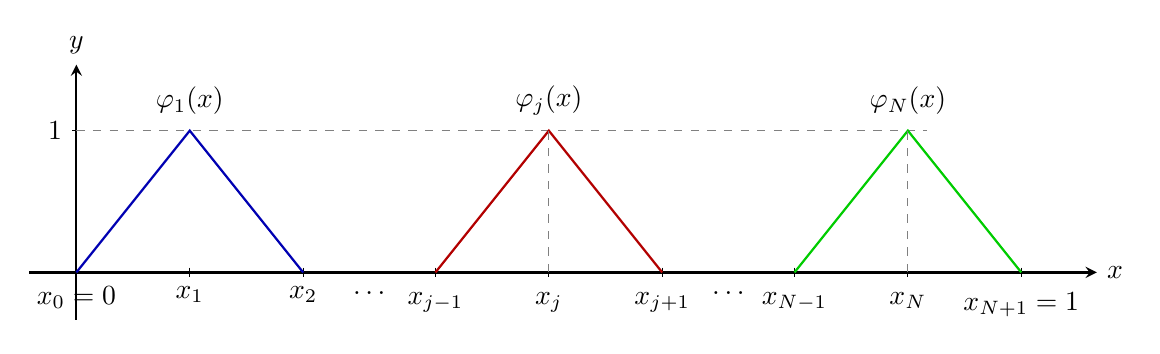
\begin{tikzpicture}[scale=1.2, >=stealth]
  % Définition des styles pour la clarté du code
  \tikzset{
    axis/.style={->, thick},
    hat1/.style={thick, blue!70!black},
    hatj/.style={thick, red!70!black},
    hatN/.style={thick, green!80!black},
    guide/.style={dashed, gray, thin},
    tick/.style={black, thin}
  }

  % Axes (allongés pour accueillir la fin du maillage)
  \draw[axis] (-0.5,0) -- (10.8,0) node[right] {$x$};
  \draw[axis] (0,-0.5) -- (0,2.2) node[above] {$y$};

  % Hauteur unitaire (y = 1) graphiquement calée à 1.5 cm
  \draw[tick] (0.05, 1.5) -- (-0.05, 1.5) node[left] {$1$};
  \draw[guide] (0, 1.5) -- (9.0, 1.5);

  % --- Graduation des nœuds (Pas constant h = 1.2) ---
  
  % Section initiale
  \draw[tick] (0,0.05) -- (0,-0.05) node[below] {$x_0=0$};
  \draw[tick] (1.2,0.05) -- (1.2,-0.05) node[below] {$x_1$};
  \draw[tick] (2.4,0.05) -- (2.4,-0.05) node[below] {$x_2$};
  
  \node[below] at (3.1,-0.1) {$\dots$};

  % Section générique j
  \draw[tick] (3.8,0.05) -- (3.8,-0.05) node[below=2pt] {$x_{j-1}$};
  \draw[tick] (5.0,0.05) -- (5.0,-0.05) node[below=2pt] {$x_j$};
  \draw[tick] (6.2,0.05) -- (6.2,-0.05) node[below=2pt] {$x_{j+1}$};
  
  \node[below] at (6.9,-0.1) {$\dots$};

  % Section finale N
  \draw[tick] (7.6,0.05) -- (7.6,-0.05) node[below=2pt] {$x_{N-1}$};
  \draw[tick] (8.8,0.05) -- (8.8,-0.05) node[below=2pt] {$x_N$};
  \draw[tick] (10.0,0.05) -- (10.0,-0.05) node[below=2pt] {$x_{N+1}=1$};

  % --- Tracé des fonctions chapeaux ---
  
  % Fonction \varphi_1(x)
  \draw[hat1] (0,0) -- (1.2,1.5) node[above, black, yshift=2pt] {$\varphi_1(x)$} -- (2.4,0);
  
  % Fonction \varphi_j(x)
  \draw[hatj] (3.8,0) -- (5.0,1.5) node[above, black, yshift=2pt] {$\varphi_j(x)$} -- (6.2,0);
  
  % Fonction \varphi_N(x) (Part de N-1, pic en N, s'éteint en N+1)
  \draw[hatN] (7.6,0) -- (8.8,1.5) node[above, black, yshift=2pt] {$\varphi_N(x)$} -- (10.0,0);

  % Lignes de rappel verticales pour les sommets internes
  \draw[guide] (5.0,0) -- (5.0,1.5);
  \draw[guide] (8.8,0) -- (8.8,1.5);

\end{tikzpicture}
\caption{Représentation schématique des fonctions de base chapeau $\varphi_j(x)$ (Éléments Finis $P_1$).}
\label{fig:hat_functions}
\end{figure}

L'expression analytique de la fonction chapeau $\varphi_j(x)$ s'écrit :
\begin{equation}
\varphi_j(x) = \begin{cases} 
\frac{x - x_{j-1}}{h} & \text{si } x_{j-1} \le x \le x_j \\ 
\frac{x_{j+1} - x}{h} & \text{si } x_j \le x \le x_{j+1} \\ 
0 & \text{sinon} 
\end{cases}
\end{equation}

Les dérivées de ces fonctions de base sont constantes par morceaux :
\begin{equation}
\varphi_j'(x) = \begin{cases} 
\frac{1}{h} & \text{si } x_{j-1} < x < x_j \\ 
-\frac{1}{h} & \text{si } x_j < x < x_{j+1} \\ 
0 & \text{sinon} 
\end{cases}
\end{equation}

\begin{figure}[H]
\centering
\begin{tikzpicture}[scale=1.2]
  % Axes
  \draw[->, thick] (-0.5,0) -- (6.5,0) node[right] {$x$};
  \draw[->, thick] (0,-1.5) -- (0,1.5) node[above] {$y$};

  % Graduation nœuds
  \draw (0,0.1) -- (0,-0.1) node[below] {$x_0$};
  \draw (1.5,0.1) -- (1.5,-0.1) node[below] {$x_{j-1}$};
  \draw (3.5,0.1) -- (3.5,-0.1) node[below] {$x_j$};
  \draw (5.5,0.1) -- (5.5,-0.1) node[below] {$x_{j+1}$};

  % Dérivée phi_j'
  \draw[very thick, remfr] (0,0) -- (1.5,0);
  \draw[very thick, remfr] (1.5,0.8) -- (3.5,0.8) node[above, midway] {$\varphi_j'(x) = \frac{1}{h}$};
  \draw[very thick, remfr] (3.5,-0.8) -- (5.5,-0.8) node[below, midway] {$\varphi_j'(x) = -\frac{1}{h}$};
  \draw[very thick, remfr] (5.5,0) -- (6.5,0);

  % Lignes de discontinuité dashed
  \draw[dashed, gray] (1.5,0) -- (1.5,0.8);
  \draw[dashed, gray] (3.5,0.8) -- (3.5,-0.8);
  \draw[dashed, gray] (5.5,-0.8) -- (5.5,0);
\end{tikzpicture}
\caption{Représentation de la dérivée première $\varphi_j'(x)$ de la fonction chapeau.}
\label{fig:derivative_hat}
\end{figure}

\subsection{Calcul de la matrice de rigidité et du second membre}

Calculons les coefficients $A_{ij} = \int_{0}^{1} \varphi_i'(x) \varphi_j'(x) \, dx$ :
\begin{itemize}
    \item \textbf{Cas $i = j$ (Diagonale) :}
    $$A_{j,j} = \int_{x_{j-1}}^{x_{j+1}} (\varphi_j'(x))^2 \, dx = \int_{x_{j-1}}^{x_j} \left(\frac{1}{h}\right)^2 \, dx + \int_{x_j}^{x_{j+1}} \left(-\frac{1}{h}\right)^2 \, dx = \frac{1}{h^2}(h) + \frac{1}{h^2}(h) = \frac{2}{h}$$
    
    \item \textbf{Cas $i = j-1$ (Sous-diagonale) :}
    $$A_{j-1,j} = \int_{x_{j-1}}^{x_j} \varphi_{j-1}'(x) \varphi_j'(x) \, dx = \int_{x_{j-1}}^{x_j} \left(-\frac{1}{h}\right)\left(\frac{1}{h}\right) \, dx = -\frac{1}{h^2}(h) = -\frac{1}{h}$$
    
    \item \textbf{Cas $i = j+1$ (Sur-diagonale) :}
    $$A_{j+1, j} = \int_{x_j}^{x_{j+1}} \varphi_{j+1}'(x) \varphi_j'(x) \, dx = \int_{x_j}^{x_{j+1}} \left(\frac{1}{h}\right)\left(-\frac{1}{h}\right) \, dx = -\frac{1}{h^2}(h) = -\frac{1}{h}$$
    
    \item \textbf{Cas $|i-j| > 1$ :}
    Puisque les supports de $\varphi_i$ et $\varphi_j$ ne s'intersectent pas (d'intersection presque partout nulle), on obtient immédiatement :
    $$A_{ij} = 0$$
\end{itemize}

La matrice de rigidité globale $A \in \mathbb{R}^{N \times N}$ est donc une matrice tridiagonale hautement creuse de la forme suivante :
\begin{equation}
A = \frac{1}{h} \begin{bmatrix}
2 & -1 & 0 & \dots & 0 \\
-1 & 2 & -1 & \ddots & \vdots \\
0 & -1 & 2 & \ddots & 0 \\
\dots & \ddots & \ddots & \ddots & -1 \\
0 & \dots & 0 & -1 & 2
\end{bmatrix}
\end{equation}

Calculons à présent les composantes du vecteur second membre $f_i$ :
$$f_i = \int_{0}^{1} f(x) \varphi_i(x) \, dx = \int_{x_{i-1}}^{x_{i+1}} f(x)\varphi_i(x) \, dx = \int_{x_{i-1}}^{x_i} f(x) \varphi_i(x) \, dx + \int_{x_i}^{x_{i+1}} f(x) \varphi_i(x) \, dx$$

Si l'on ne peut pas intégrer de manière analytique exacte ces intégrales, on emploie la \textbf{méthode des trapèzes} sur chacun de ces deux intervalles d'intégration pour approximer numériquement le résultat :
$$\int_{x_{i-1}}^{x_i} f(x)\varphi_i(x) \, dx \approx \frac{h}{2} \Big( f(x_{i-1})\underbrace{\varphi_i(x_{i-1})}_{=0} + f(x_i)\underbrace{\varphi_i(x_i)}_{=1} \Big) = \frac{h}{2} f(x_i)$$
$$\int_{x_i}^{x_{i+1}} f(x)\varphi_i(x) \, dx \approx \frac{h}{2} \Big( f(x_i)\underbrace{\varphi_i(x_i)}_{=1} + f(x_{i+1})\underbrace{\varphi_i(x_{i+1})}_{=0} \Big) = \frac{h}{2} f(x_i)$$

En additionnant ces deux contributions, on obtient l'approximation suivante du second membre :
\begin{equation}
f_i \approx \frac{h}{2} f(x_i) + \frac{h}{2} f(x_i) = h f(x_i)
\label{eq:f_trapez}
\end{equation}

En réinjectant (\ref{eq:f_trapez}) dans le système linéaire $A \vec{u} = \vec{f}$, on retrouve :
$$\frac{-u_{i-1} + 2u_i - u_{i+1}}{h} = h f(x_i) \iff \frac{-u_{i-1} + 2u_i - u_{i+1}}{h^2} = f(x_i)$$
On constate ainsi une équivalence remarquable avec le système issu des différences finies (DF).

\subsection{Comparaison : Éléments Finis (EF) vs Différences Finies (DF)}

\begin{exemple}[Avantages comparatifs des Éléments Finis]
Bien que le système discret linéaire obtenu soit identique dans ce cas unidimensionnel académique simple avec la formule des trapèzes, les Éléments Finis apportent une rigueur et une souplesse considérables par rapport aux Différences Finies :
\begin{itemize}
    \item \textbf{Plus grande liberté géométrique :} La MEF gère très naturellement les maillages non uniformes en 1D ainsi que les géométries bidimensionnelles ou tridimensionnelles extrêmement complexes (triangles, tétraèdres).
    \item \textbf{Moindre exigence de régularité :} La méthode ne requiert pas de régularité forte sur la solution ($C^4$ pour les DF) ni sur le second membre $f$.
    \item \textbf{Estimations d'erreurs plus faibles :} Les estimations de convergence sont exprimées en norme d'énergie (norme $H^1$ ou $L^2$) beaucoup plus adaptées à la physique plutôt qu'en norme infinie $C^0$ ponctuelle.
    \item \textbf{Adaptivité locale :} Elle permet de raffiner localement le maillage (ajouter plus d'éléments là où la solution varie brutalement et moins là où elle est lisse) de manière très naturelle.
\end{itemize}
\end{exemple}

\subsubsection{Synthèse graphique : DF vs EF}

Cette figure résume la différence fondamentale de philosophie entre l'approche purement discrète ponctuelle (DF) et l'approche variationnelle géométrique (EF).

\begin{figure}[H]
    \centering
    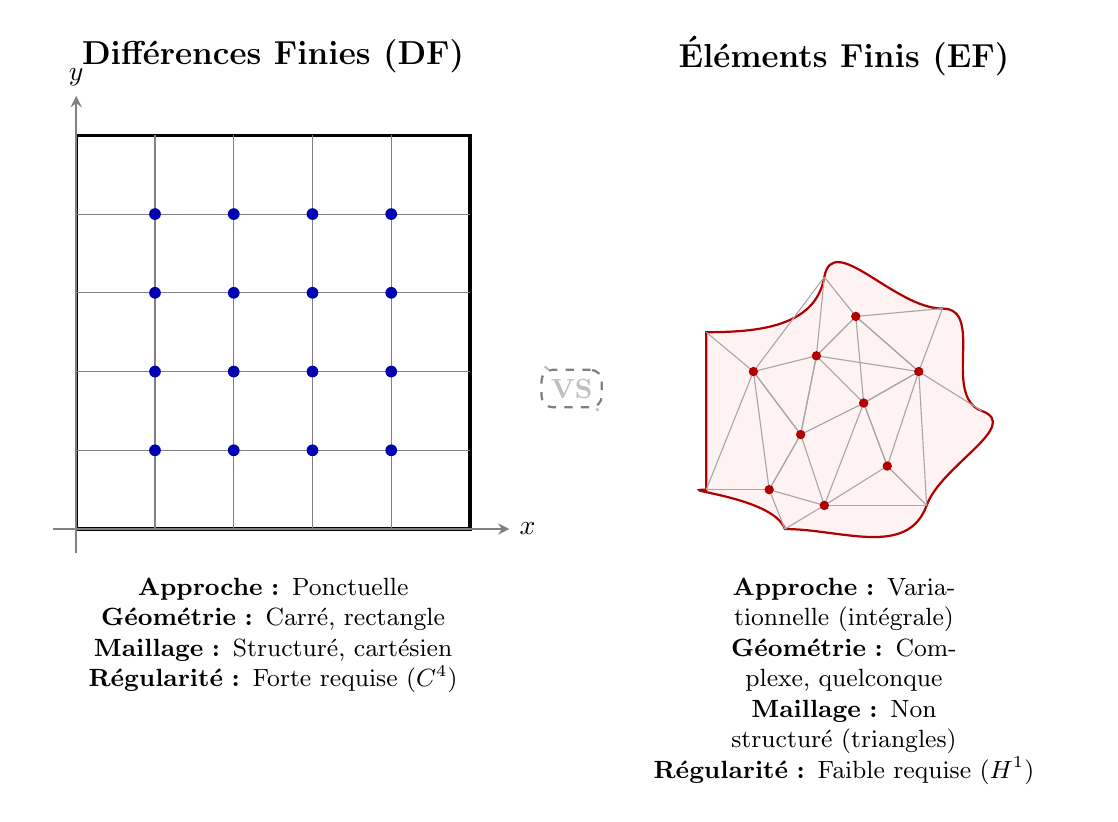
\begin{tikzpicture}[scale=1, >=stealth]
        % --- Définition des styles ---
        \tikzset{
            title/.style={font=\bfseries\large, align=center, text width=6cm},
            desc/.style={font=\small, align=center, text width=5cm},
            fd_grid/.style={gray, thin},
            fd_node/.style={circle, fill=blue!70!black, inner sep=1.5pt},
            fe_boundary/.style={thick, draw=red!70!black, fill=red!5},
            fe_mesh/.style={gray!70, thin},
            fe_node/.style={circle, fill=red!70!black, inner sep=1.2pt}
        }

        % =====================================================================
        % BLOC GAUCHE : DIFFÉRENCES FINIES (DF)
        % =====================================================================
        \begin{scope}[local bounding box=boxFD]
            % Titre
            \node[title] (titreFD) at (2.5, 6) {Différences Finies (DF)};

            % Contour du "tableau" / Domaine carré
            \draw[very thick] (0,0) rectangle (5,5);

            % Axes perpendiculaires (repère local)
            \draw[->, gray, thick] (-0.3,0) -- (5.5,0) node[right, black] {$x$};
            \draw[->, gray, thick] (0,-0.3) -- (0,5.5) node[above, black] {$y$};

            % Maillage structuré (perpendiculaire)
            \foreach \i in {1,2,3,4} {
                \draw[fd_grid] (\i, 0) -- (\i, 5); % Verticales
                \draw[fd_grid] (0, \i) -- (5, \i); % Horizontales
            }

            % Nœuds intérieurs (Points de calcul)
            \foreach \x in {1,2,3,4} {
                \foreach \y in {1,2,3,4} {
                    \node[fd_node] at (\x,\y) {};
                }
            }

            % Description textuelle
            \node[desc, anchor=north] at (2.5, -0.5) {
                \textbf{Approche :} Ponctuelle\\
                \textbf{Géométrie :} Carré, rectangle\\
                \textbf{Maillage :} Structuré, cartésien\\
                \textbf{Régularité :} Forte requise ($C^4$)
            };
        \end{scope}

        % =====================================================================
        % BLOC DROIT : ÉLÉMENTS FINIS (EF)
        % =====================================================================
        \begin{scope}[shift={(8,0)}, local bounding box=boxEF]
            % Titre
            \node[title] (titreEF) at (1.75, 6) {Éléments Finis (EF)};

            % Forme quelconque avec arrondis (Blob)
            \path[fe_boundary] 
                (0,0.5) to[out=180,in=110] (1,0)
                to[out=0,in=250] (2.8,0.3)
                to[out=70,in=340] (3.5,1.5)
                to[out=160,in=0] (3,2.8)
                to[out=180,in=80] (1.5,3.2)
                to[out=260,in=0] (0,2.5) -- cycle;
            
            % --- Triangle Mesh (Manuel mais représentatif) ---
            \coordinate (A) at (0.8, 0.5);
            \coordinate (B) at (1.5, 0.3);
            \coordinate (C) at (2.3, 0.8);
            \coordinate (D) at (1.2, 1.2);
            \coordinate (E) at (2.0, 1.6);
            \coordinate (F) at (2.7, 2.0);
            \coordinate (G) at (0.6, 2.0);
            \coordinate (H) at (1.4, 2.2);
            \coordinate (I) at (1.9, 2.7);
            
            \coordinate (b1) at (0, 0.5); \coordinate (b2) at (1, 0); \coordinate (b3) at (2.8, 0.3);
            \coordinate (b4) at (3.5, 1.5); \coordinate (b5) at (3, 2.8); \coordinate (b6) at (1.5, 3.2);
            \coordinate (b7) at (0, 2.5);

            % Dessin des arrêtes (Mesh)
            \draw[fe_mesh] (A)--(B)--(D)--cycle;
            \draw[fe_mesh] (B)--(C)--(E)--cycle;
            \draw[fe_mesh] (C)--(F)--(E)--cycle;
            \draw[fe_mesh] (D)--(E)--(H)--cycle;
            \draw[fe_mesh] (E)--(F)--(I)--cycle;
            \draw[fe_mesh] (G)--(H)--(D)--cycle;
            \draw[fe_mesh] (H)--(I)--(F)--cycle;
            \draw[fe_mesh] (A)--(D)--(G)--cycle;
            
            % Connections aux bords
            \draw[fe_mesh] (A)--(b1); \draw[fe_mesh] (A)--(b2); \draw[fe_mesh] (B)--(b2); \draw[fe_mesh] (B)--(b3);
            \draw[fe_mesh] (C)--(b3); \draw[fe_mesh] (F)--(b3); \draw[fe_mesh] (F)--(b4); \draw[fe_mesh] (F)--(b5);
            \draw[fe_mesh] (I)--(b5); \draw[fe_mesh] (I)--(b6); \draw[fe_mesh] (H)--(b6); \draw[fe_mesh] (G)--(b6);
            \draw[fe_mesh] (G)--(b7); \draw[fe_mesh] (G)--(b1);
            
            % Nœuds intérieurs (Points de calcul)
            \foreach \p in {A,B,C,D,E,F,G,H,I} {\node[fe_node] at (\p) {};}

            % Description textuelle
            \node[desc, anchor=north] at (1.75, -0.5) {
                \textbf{Approche :} Variationnelle (intégrale)\\
                \textbf{Géométrie :} Complexe, quelconque\\
                \textbf{Maillage :} Non structuré (triangles)\\
                \textbf{Régularité :} Faible requise ($H^1$)
            };
        \end{scope}

        % =====================================================================
        % SÉPARATEUR CENTRAL (Bypasse l'erreur calc via l'ancrage 'midway')
        % =====================================================================
        \draw[dashed, gray!50, thick] (boxFD.east) -- (boxEF.west) 
            node[midway, fill=white, rounded corners, draw=gray, font=\bfseries] {VS};

    \end{tikzpicture}
    \caption{Comparaison des approches de discrétisation spatiale : rigidité structurée des Différences Finies (à gauche) contre flexibilité géométrique des Éléments Finis triangulaires (à droite).}
    \label{fig:comparison_df_ef}
\end{figure}